\chapter{Grundlagen}
\label{chapter:basics}

Im Folgenden sollen Verfahren und Techniken %hier thmea nochmal angreifen ,techniken wofür etc.
erläutert werden, welche für das Verständnis der späteren Kapitel essenziell sind.
Dafür werden die relevanten Hardwarekomponenten und Vorausetzungen an die Caches erklärt.
Zudem werden grundlegende Cache-Angriffe wie Prime-and-Probe sowie Flush-and-Reload vorgestellt.
Weiterhin werden die mathematischen Grundlagen für die spätere Leakage-Analyse von RSA beschrieben.

%\todo[size=\footnotesize]{Hier sollte mehr stehen als ein Satz, ergibt sich vielleicht später. Hier gehört die Erklärung des Themas hin sowie eine Bestimmung der Rewlevanz des Themas für die Forschung.} 
%\todo[size=\footnotesize]{Generell: Du tendierst zu verschachtelten und langen Sätzen. Versuche, Simplere Sätze mit höchstens einem Komma und ohne Zwischeneinschübe zu verwenden. }
\section{Virtuelle Speicherverwaltung}

%Quelle von Tannenbaum eingefügt
%\todo[size=\footnotesize]{Ein Quelle in Absatz einfügen?}

Virtuelle Speicherverwaltung stellt eine Abstraktion für die vorhandenen physischen Speichermedien wie etwa den Hauptspeicher oder die Festplatte bereit \cite{tanenbaumVirtualMemory}.
Das Betriebssystem übersetzt virtuelle Adressen, welche von Prozessen genutzt werden, mit Hilfe der Hardware in physische Adressen. 
Jedem Prozess steht der gleiche virtuelle Adressraum zur Verfügung, wobei das Betriebssystem dafür Sorge trägt, dass für jeden Prozess die richtige Zuordnung von virtueller zu physischer Adresse sichergestellt wird.
Ein Vorteil der virtuellen Speicherverwaltung ist eine erhöhte Sicherheit durch die Speicherisolierung aller Prozesse, da ein Prozess keinen Zugriff auf das Adressmapping eines anderen hat.
So kann eine fehlerhafte Schreiboperation eines Prozesses keinen Fehler in anderen Prozessen verursachen, da gleiche virtuelle Adressen vom Betriebssystem auf unterschiedliche physische Adressen abgebildet werden.
%Des Weiteren kann ein Prozess mehr Hauptspeicher nutzen als physisch vorhanden ist, indem Daten vom Betriebssystem auf andere Speichermedien wie die Festplatte ausgelagert werden. Hiermit werden beispielsweise Anwendungsentwickler entlastet, da sie ihre Software nicht für Systeme mit weniger Hauptspeicher gesondert anpassen müssen. 

%Speicher-Deduplizierung wird in der Arbeit nicht weiter erwähnt, deswegen würde ich es hier auch nicht beschreiben.
%\todo[size=\footnotesize]{ggf. Speicher-Deduplizierung, wo du dann plötzlich doch das gleiche Mapping hast. }

\section{Caches}

Die Geschwindigkeitsentwicklung des Hauptspeichers konnte in den letzten Jahren nicht mit der des Prozessors Schritt halten \cite{speedGapCPUandRAM}. Der Cache ist ein im Vergleich zum Hauptspeicher kleinerer, aber schnellerer Pufferspeicher, welcher im aktuellen Kontext häufig benötigte Daten vorhält. Diese Daten zeichnen sich auch häufig dadurch aus, dass sie räumlich nah beieinander liegen.
Ohne Caches wäre ein Prozessor häufig gezwungen, auf Daten des langsamen Hauptspeichers zu warten, und würde in seiner Verarbeitungsgeschwindigkeit gebremst. %\todo[size=\footnotesize]{positiv formulieren: Mit cache muss man nicht warten, dadurch wirds schneller} Ist die Aussage nicht wirkungsgleich beziehungsweise genauso Pro-Caches vormuliert?
Weiter liegt der Fokus der Arbeit auf der im Desktopbereich weit verbreiteten x86-Architektur. Deshalb werden mit Intel-Prozessoren der Core-Architektur bestückte Testrechner verwendet, da Intels Core-Architektur im x86-Desktopsegment zurzeit den höchsten Marktanteil besitzt \cite{AMDIntelMarketShare}. Aus diesem Grund werden Erklärungen im Folgenden häufig mit Beispielen der Intel Core-Architektur veranschaulicht.

Ein Cache der Core-Architektur lagert nicht einzelne Bytes, sondern immer gleich 64 Bytes, Cache-Line genannt, auf einmal ein. Dabei werden die 64 Bytes beginnend ab der größten Adresse, welche zugleich kleiner als die Zieladresse und ein Vielfaches von 64 ist, angefragt.
Angenommen 4 Bytes Daten an Adresse \lstinline!0b10110111!
werden angefordert, dann lagert der Cache die 64 Bytes beginnend mit der Adresse \lstinline!0b10000000! ein.
Heutige Arbeitsspeichermodule liefern 8 Bytes zeitgleich, wobei die CPU mit einem einzigen Befehl einen Burst von 8 Übertragungen initiieren kann, die das Lesen und Schreiben einer gesamten 64-Bytes-Cache-Line ermöglichen.
Das Vorausladen von aktuell nicht benötigten Daten liegt in der Lokalitätseigenschaft typischer Programme begründet \cite{tanenbaumLocality}. So besagt die zeitliche Lokalität, dass aktuell verwendete Daten mit hoher Wahrscheinlichkeit in naher Zukunft erneut benötigt werden. Räumliche Lokalität hingegen besagt, dass beim Zugriff einer bestimmten Speicheradresse benachbarte Speicheradressen in naher Zukunft mit hoher Wahrscheinlichkeit benötigt werden.
Somit ist es von Vorteil, gleichzeitig 64 Bytes zu laden, da die zusätzlich geladenen Bytes mit hoher Wahrscheinlichkeit in den nächsten Zyklen ebenfalls benötigt werden. Der Performancenachteil, welcher durch ein Laden von gleichzeitig 64 Bytes entsteht, ist im Gegensatz dazu vernachlässigbar.

Ein Prozessorcache besteht üblicherweise aus mehreren Ebenen, Cache-Levels genannt, wobei die Core-Architektur etwa 3 Cache-Levels besitzt, welche absteigend größer und langsamer werden. Ein Intel i7-4770 besitzt pro physischem Kern beispielsweise einen 32 KiB-L1-Datencache mit einer Zugriffslatenz von 4 bis 5 Taktzyklen und einen 256 KiB-L2-Cache mit einer Latenz von 12 Taktzyklen \cite{CacheStatsHaswell}.
Im Unterschied zu den beiden ersten Cache-Levels teilen sich in der Core-Architektur alle Kerne den L3-Cache. 
Dies bedeutet aus Sicht der Angreiferin einen großen Vorteil, da jedes Programm den Zustand des L3-Caches beeinflusst, und zwar unabhängig davon, auf welchem Kern es ausgeführt wird.
Dagegen muss die Angreiferin bei einem Angriff auf den L1- beziehungsweise L2-Cache sicherstellen, dass ihr Code und das angegriffene Programm auf demselben physischen Kern ausgeführt werden.

Die Ersetzungsstrategie legt fest, welcher Eintrag aus dem Cache verdrängt wird, sofern alle Einträge des zugehörigen Cache-Sets belegt sind. 
Intels Core-Prozessoren verdrängen typischerweise den Eintrag, welcher bezogen auf die letzte Zugriffszeit am ältesten ist, auch least-recently-used-Strategie (LRU) genannt. 
Ab der Ivy-Bridge-Generation passt Intel diese Strategie situationsbedingt an \cite{CacheReplacementPolicy} und verwendet ebenfalls  die bimodul insertion policy (BIP), welche häufig den zuletzt hinzugefügten Eintrag löscht. 
Dies kann von Vorteil sein, wenn das Working-Set des Programms die Größe des Caches übersteigt und die LRU-Strategie zu keinen Cache-Hits führen würde.
Bei Ivy-Bridge Prozessoren stellten die Autoren des Papers fest, dass manche Cache-Sets die LRU-Strategie und manche die BIP-Strategie verfolgen. 
Es wird daher ein Echtzeitvergleich zwischen beiden Strategien vermutet, um herauszufinden, welche Strategie weniger Cache-Misses produziert. 
Bei den Nachfolger- Generationen Haswell und Broadwell stellten die Autoren fest, dass zwischen beiden Strategien mit hoher Frequenz gewechselt wird, wobei der Algorithmus hinter den Ersetzungsstrategien ebenfalls nicht öffentlich zugänglich ist.

\subsection{Assoziativität}

%\newtext

Sofern die Auswahl des Cache-Eintrags für die Daten einer bestimmten Hauptspeicheradresse keinerlei Beschränkungen unterliegt, wird von einem voll-assoziativen Cache gesprochen. 
Das andere Extrem wäre ein einfach-assoziativer Cache beziehungsweise eine direkte Abbildung, wobei die Adresse des Hauptspeichers, von der die Daten stammen, den zu wählenden Cache-Eintrag eindeutig festlegt.
Der Mittelweg ist die n-Wege-Assoziativität, bei der die Daten nur an n Cache-Einträgen liegen können (siehe auch Abb. \ref{fig:CacheAsso}).

%\todo{Tabellen haben Überschriften, Abbildungen haben Unterschriften. Bitte für alle Abbildungen unter das Bild schieben.}
\label{fig:CacheAsso}
\begin{figure}[h]
\centering
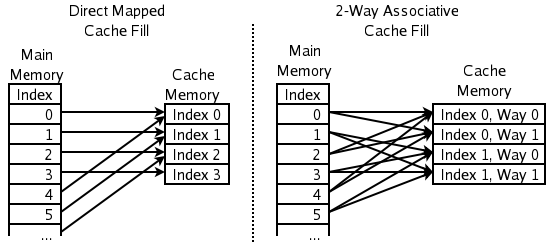
\includegraphics[width=0.8\textwidth]{basics/Cache_Asso.png}
\caption{Links ist ein direkt abgebildeter Cache zu sehen, bei dem die Hauptspeicheradresse den Cache-Index vollumfänglich festlegt. Rechts ist ein 2-Wege assoziativer Cache zu sehen bei dem etwa die Hauptspeicheradresse 0 sowohl auf \textit{Index 0, Way 0} als auch auf \textit{Index 0, Way 1} im Cache abgebildet werden kann \cite{CacheAssoWiki}.}
\end{figure}

%\newtextend

Der L3-Cache eines Intel i7-4770 ist beispielsweise 8 MiB groß und verfügt daher über 131072 ($2^{17}$) Cache-Einträge in der Größe einer Cache-Line. 
Wäre dieser Cache nun voll-assoziativ, müsste er bei jeder Anfrage komplett durchsucht werden. Aus diesem Grund ist der Cache in Cache-Sets unterteilt, wobei Daten einer spezifischen Hauptspeicheradresse nur in genau ein Cache-Set eingelagert werden können. 
Der i7-4770 besitzt 8192 dieser Cache-Sets, womit sich eine Assoziativität von 16 ergibt, das heißt man teilt die Anzahl der Cache-Einträge durch Anzahl der Cache-Sets. Dies bedeutet, dass die Suche nach den Daten einer Hauptspeicheradresse im Cache auf 16 Einträge begrenzt ist. 
%Die Zuordnung der physischen Hauptspeicheradressen zu den Cache-Sets ist nicht öffentlich dokumentiert.
Des Weiteren wird der Cache in \textit{Slices} unterteilt, wobei jede Slice einem Kern zugeordnet wird. Die Slices sind mittels eines Ringbuses verbunden, so dass jeder Kern auf Daten jeder Slice zugreifen kann. Die Zugriffslatenz erhöht sich mit der Anzahl der benötigten Hops, jedoch ist diese Erhöhung im Bereich von etwa 10 ns pro Hop. Diese Latenzunterschiede sind daher zu gering, um die Erkennung zwischen Cache-Hit und Cache-Miss zu gefährden, welche bei ca. 60 ns liegen \cite{TheSpyInTheSandbox}. Bei i7-4770 sind jedem der 4 Slices 2048 Cache-Sets zugeordnet. Die Zuordnung der Cache-Sets innerhalb der Slices sind fest an die untersten 18 Bit der pysischen Adresse gekoppelt. Zu welchem Slice eine Adresse gemappt wird, wird durch eine nicht dokumentierte Hashfunktion bestimmt.

%Im Rahmen dieser Arbeit sind Slices daher vernachlässigbar, so dass etwa bei Cache-Spezifikationen Slices nicht gesondert erwähnt werden.
%\todo[size=\footnotesize]{Eventuell Slices doch nicht so vernachlässigbar, da store forward eviction set Suche Slices einbezieht)}



%\todo[size=\footnotesize]{Hier fehlt wieder Mapping durch letzte Bits der Adresse (Beschrieben in Abschnitt Prime-and-Probe)}

%Ein CPU-Cache enthält mehrere Einträge, welche folgende Bestandteile besitzen:
%\begin{enum}
%\item Cache-Line: Die gecacheten Daten, wobei die Länge in der Core-Architektur etwa 64 Bytes beträgt.
%\item Address-Tag: Die Adresse im Hauptspeicher von der die Daten in der Cache-Line stammen.
%\item Flag-Bits: Etwa das "Dirty"-Bit welches anzeigt ob die Daten der Cache-Line noch mit denen im Hauptspeicher übereinstimmen.
%\end{enum}

\subsection{\textit{Inclusive} und \textit{exclusive}}
Ein Cache wird als \textit{inclusive} bezeichnet, falls alle Daten, die in einem niedrigen Cache-Level vorliegen, zusätzlich auch in den höheren Cache-Levels eingelagert sind. 
So besitzen die Caches aller Desktop-Versionen der Intel Core-Architektur diese inclusive-Eigenschaft (Stand Juni 2018).
Die Caches der Desktop-Prozessoren des Konkurrenten AMD haben zum Beispiel die Zen-Architektur \cite{CacheRyzen}, während jene der aktuellen Skylake-X-Prozessoren \cite{CacheSkylakeX} für Intels High-Performance-Plattform diese Eigenschaft hingegen nicht besitzen.
Wegen des großen Marktanteils von Intel-CPUs kann festgehalten werden, dass der Großteil der sich im Einsatz befindlichen Prozessoren mit \textit{Inclusive}-Caches ausgestattet ist.

\section{Cache-Angriffe}

Cache-Angriffe beschreiben eine generelle Klasse von Mikro\-architektur-Seiten\-kanal\-angriffen, welche den Cache verwenden, um Informationen abzugreifen, wobei der Cache als geteilte Ressource zwischen verschiedenen Prozessen fungiert. Durch diesen Angriff können sichere und unsichere Prozesse über den geteilten Cache trotz höher liegender Schutzmechanismen wie virtualisiertem Speicher oder Hypervisor-Systemen kommunizieren. 
Eine Angreiferin könnte ein Programm entwickeln, welches Informationen über den inneren Zustand eines anderen Prozesses sammelt, und so AES-Schlüssel \cite{BernsteinAES} sowie RSA-Schlüssel \cite{CacheAttackRSA} abgreifen auch über die Grenzen von virtuellen Maschinen hinweg.

%\newtext

\subsection{Flush-and-Reload}

Diese Angriffstechnik wurde 2014 von Yuval Yarom
und Katrina Falkner veröffentlicht \cite{FlushReload}.
Ausgang dieses Angriffs ist ein architekturspezifischer Flush-Befehl wie etwa der x86-Assemblerbefehl \textit{clflush}, welcher eine Adresse entgegennimmt und die dazugehörige Cache-Line invalidiert. 
Dadurch müssen die Daten beim nächsten Zugriff aus dem Hauptspeicher geladen werden. Dies ist die erste Phase des Angriffs und wird als Flush bezeichnet. 

Nach dem Flush folgt die Wait-Phase, in welcher die Angreiferin eine bestimmte Zeitperiode wartet und anschließend die Zugriffszeit auf die geflushte Adressse misst. 

Zu guter Letzt folgt die Reload-Phase, in welcher die Angreiferin auf die Adresse zugreift. Sofern das Opferprogramm in der Wait-Phase auf die Adresse zugegriffen hat, ist die Zugriffszeit gering, da die Daten bereits im Cache vorliegen.
Im anderen Fall müssen die Daten erst aus dem Hauptspeicher geladen werden, womit eine messbar erhöhte Zugriffszeit einhergeht \cite{FlushReload}. Eine Übersicht der eben beschriebenen Schritte als Pseudocode findet sich in Algorithmus \ref{alg:flush_and_reload}.

Ein Nachteil dieser Angriffsmethode ist die Notwendigkeit, dass sich der Opferprozess Speicherseiten mit dem Prozess der Angreiferin teilen muss. 
Ein typisches Beispiel hierfür sind geteilte Bibliotheken, zum Beispiel .so Dateien unter Linux oder .dll Dateien unter Windows, welche etwa Kryptofunktionen bereitstellen. Des Weiteren ist der clflush-Befehl nicht in jeder Umgebung verfügbar. So ist etwa ein Angriff aus dem Browser heraus mit dieser Methode nicht möglich. 
%\todo[size=\footnotesize]{Du hast ja schon geschrieben todo. Hier vielleicht auch eine kleine abbildung, aber defintiv irgendwas über flush WAIT reload und zeitmessungen}


%\todo{Ok, ich sehe du benutzt keine listing-Umgebung, sondern das alogrithm(2) Paket. Dann habe ich keine Ahnung, wie du die Schriftgröße anpassen kannst. Musst du dann selber rausfinden.}
\SetKwProg{Fn}{Function}{}{}

\begin{algorithm}[h]
\DontPrintSemicolon
\caption{Pseudo-Code für Flush-and-Reload}
\label{alg:flush_and_reload}
\SetAlgoNlRelativeSize{-2}

\Fn{$flushAndReload(address)$}{
    clflush(address)\;
    wait()\;
	timestampBefore <- getTimestamp()\;
	readMem(address)\;
	timestampAfter <- getTimestamp()\;
	\Return timestampAfter - timestampBefore > threshold
}

%\newtextend

\end{algorithm}

\subsection{Prime-and-Probe}

Ein erfolgreicher Prime-and-Probe Angriff auf den L3-Cache wurde 2015 etwa von Irazoqui et al. veröffentlicht \cite{ITSPrimeAndProbe}.
Er unterscheidet sich von Prime-and-Probe Angriffen auf niedrigere Cache-Level durch die aufwendigere Eviction-Set Suche.

Ein \textit{Eviction-Set} sei eine Menge Adressen, welche einen Cache-Eintrag aus einem Cache verdrängen kann. D.h. ein Eviction-Set, welches einen Eintrag aus dem L3-Cache löscht, würde den gleichen Zweck wie der \textit {clflush}-Assemblerbefehl im Flush-and-Reload-Angriff erfüllen. 
Um einen Eintrag aus dem Cache zu verdrängen, müssen mehrere Adressen der Daten aus dem Eviction-Set von der CPU auf das gleiche Cache-Set wie der zu verdrängende Eintrag abgebildet werden, so dass die Größe eines Eviction-Sets mindestens die Assoziativität des Caches erreichen muss.

Die Idee beim Prime-and-Probe Angriff besteht darin, in einer sich wiederholenden Abfolge zuerst den Cache zu primen, dann das Opferprogramm rechnen zu lassen und anschließend zu proben.
In der Priming-Phase werden mittels der Eviction-Sets gezielt Cache-Sets vollständig mit den Daten aus dem Eviction-Set belegt.
In der anschließenden Berechnungsphase werden einige Einträge aus den geprimten Cache-Sets vom Opferprogramm verdrängt. Abschließend berechnet die Angreiferin die Summe der Zugriffszeiten auf alle Einträge in einem Eviction-Set.
Sofern das Opferprogramm in dem zum Eviction-Set korrelierenden Cache-Set Einträge verdrängt hat, kann die Angreiferin eine Abweichung nach oben in ihrer Messung feststellen, da die verdrängten Einträge eine erhöhte Zugriffszeit verursachen. Somit kann aus den Zugriffszeiten der Eviction-Sets auf die Speicherzugriffe des Opferprogramms geschlossen werden.

Die Eviction-Sets, die zur Durchführung eines Cache-Angriffs notwendig sind, lassen sich nicht immer leicht finden, da das Mapping der virtuellen auf die physischen Adressen in manchen Umgebungen nur eingeschränkt zugänglich ist.
So ist aber in der Regel das Mapping der virtuellen und physischen Adressen bei den Adressbits der Speicher-Pages identisch, welche etwa unter Windows und Linux zur Zeit 4096 Bytes groß sind. Somit ist in diesem Fall garantiert, dass die untersten 12 virtuellen Adressbits mit den physischen Adressbits identisch sind. 

%Der L3-Caches des Intel i7-4770 ist etwa 8 Mib groß, sodass 11 Bits des Mapping auf die physischen Adressen unbekannt sind.
%In solchen Fällen müssen die Eviction-Sets in einem Trial-and-Error-Verfahren ermittelt werden, wie es der Algorithmus TODO %\ref[alg:evictionSet} beschreibt.

\begin{algorithm}[h]
\DontPrintSemicolon
\caption{Pseudo-Code für Prime-and-Probe}
\label{alg:prime_and_pribe}

\Fn{$flushAndReload(address)$}{
    \ForEach{address in evictionSet}{
        readMem(address)\;
    }
    wait()\;
	timestampBefore <- getTimestamp()\;
	\ForEach{address in evictionSet}{
        readMem(address)\;
    }
	timestampAfter <- getTimestamp()\;
	\Return timestampAfter - timestampBefore > threshold
}

\end{algorithm}


%Beschreibe Algorithmus
%Hierfür werden zuerst wiederholt Speicherblöcke angefordert, wobei solche in einer Menge gesammelt werden, welche 

%\newtext

\subsection{Timer}

Beide eben beschriebenen Angriffsmethoden setzen voraus, dass die Angreiferin Laufzeitunterschiede zwischen dem Ladevorgang aus dem Cache und dem Hauptspeicher zuverlässig unterscheiden kann. Beim AIDA64-Benchmark mit einem aktuellen Intel i7-8700K ist die L3-Cache-Latenz im Mittel bei 12 ns, wobei gepaart mit DDR4-3200 CL16 RAM die Hauptspeicherlatenz im Mittel 49 ns beträgt \cite{i78700kLatency}. Somit ist eine Timer-Auflösung von unter 30 ns Voraussetzung für einen erfolgreichen Angriff. Anschaulich ist dies auch im Diagramm \ref{fig:RAMCacheLatency} zu sehen. Die Autoren verwendeten einen i7-4960HQ und haben Zugriffszeitdifferenzen für Cache-Miss und Hit von etwa 70 ns festgestellt. 
Auf dem Testsystem mit einem Intel i7-4770 und DDR3-1600 RAM konnten mittels \textit{rdtscp} durchschnittliche Zugriffswerte von 66 Taktzyklen bei einem Hit und von 248 Taktzyklen bei einen Miss festgestellt werden.

Im Folgenden wird Zeit oft in Taktzyklen gemessen, wobei sich damit immer auf die \textit{rdtscp}-Instruktion bezogen wird.
Zu beachten ist hierbei, dass der im Testsystem verbaute i7-4770 je nach Kern und Gegebenheiten wie Last, Temperatur und so weiter von seinem 3,4 GHz Basistakt abweicht.
Der Takt des \textit{rdtscp}-Timers ist jedoch immer auf den gleichen Takt \cite{IntelManualRDTSCP}, im Fall des Testsystems auf 3,4 GHz, fixiert.
Somit ergibt die Differenz von 182 Taktzyklen zwischen einem Hit und Miss auf dem Testsystem einen Zeitunterschied von 54 ns.

\label{fig:RAMCacheLatency}
\begin{figure}[h]
\centering
\begin{scaletikzpicturetowidth}{\textwidth}
% Created by tikzDevice version 0.12 on 2018-10-06 03:37:54
% !TEX encoding = UTF-8 Unicode
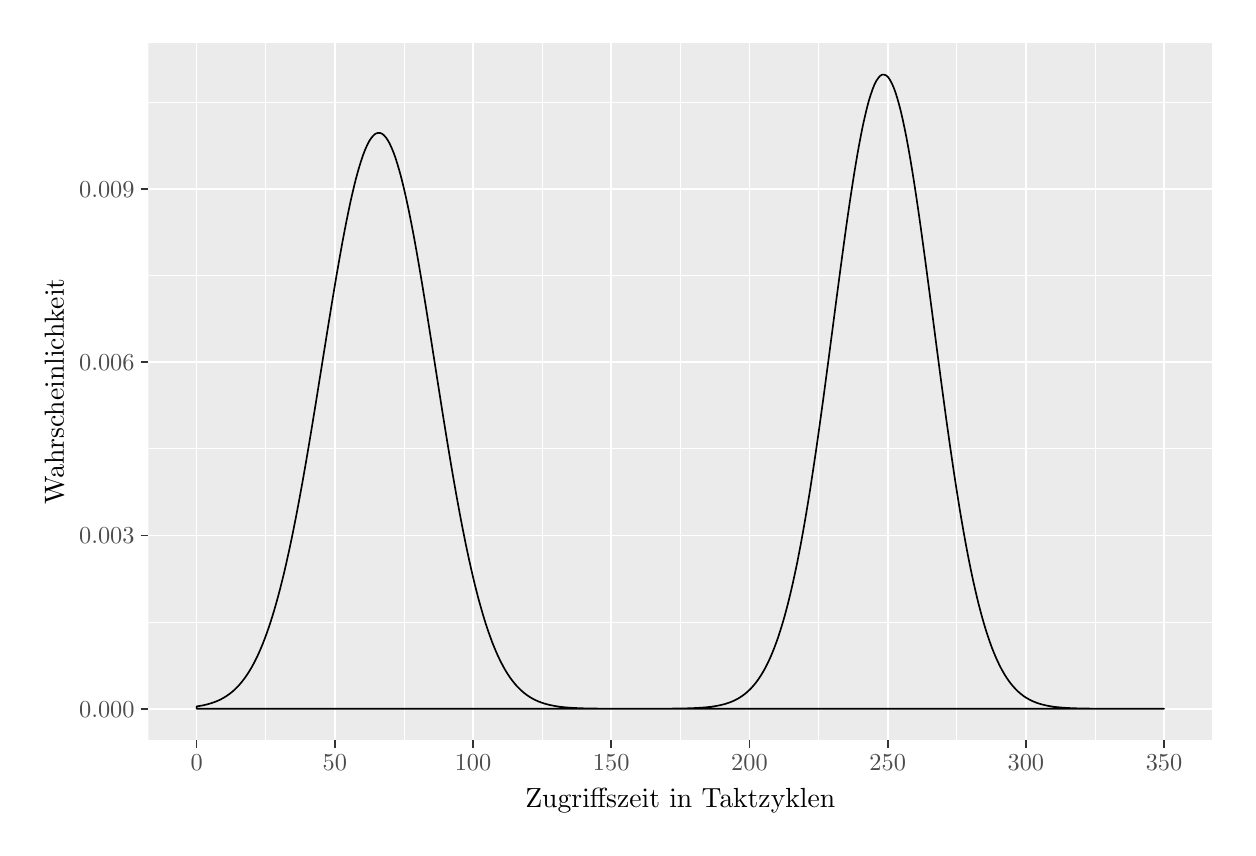
\begin{tikzpicture}[x=1pt,y=1pt]
\definecolor{fillColor}{RGB}{255,255,255}
\path[use as bounding box,fill=fillColor,fill opacity=0.00] (0,0) rectangle (433.62,289.08);
\begin{scope}
\path[clip] (  0.00,  0.00) rectangle (433.62,289.08);
\definecolor{drawColor}{RGB}{255,255,255}
\definecolor{fillColor}{RGB}{255,255,255}

\path[draw=drawColor,line width= 0.6pt,line join=round,line cap=round,fill=fillColor] (  0.00,  0.00) rectangle (433.62,289.08);
\end{scope}
\begin{scope}
\path[clip] ( 43.57, 31.53) rectangle (428.12,283.58);
\definecolor{fillColor}{gray}{0.92}

\path[fill=fillColor] ( 43.57, 31.53) rectangle (428.12,283.58);
\definecolor{drawColor}{RGB}{255,255,255}

\path[draw=drawColor,line width= 0.3pt,line join=round] ( 43.57, 74.28) --
	(428.12, 74.28);

\path[draw=drawColor,line width= 0.3pt,line join=round] ( 43.57,136.88) --
	(428.12,136.88);

\path[draw=drawColor,line width= 0.3pt,line join=round] ( 43.57,199.47) --
	(428.12,199.47);

\path[draw=drawColor,line width= 0.3pt,line join=round] ( 43.57,262.06) --
	(428.12,262.06);

\path[draw=drawColor,line width= 0.3pt,line join=round] ( 86.02, 31.53) --
	( 86.02,283.58);

\path[draw=drawColor,line width= 0.3pt,line join=round] (135.96, 31.53) --
	(135.96,283.58);

\path[draw=drawColor,line width= 0.3pt,line join=round] (185.90, 31.53) --
	(185.90,283.58);

\path[draw=drawColor,line width= 0.3pt,line join=round] (235.84, 31.53) --
	(235.84,283.58);

\path[draw=drawColor,line width= 0.3pt,line join=round] (285.78, 31.53) --
	(285.78,283.58);

\path[draw=drawColor,line width= 0.3pt,line join=round] (335.73, 31.53) --
	(335.73,283.58);

\path[draw=drawColor,line width= 0.3pt,line join=round] (385.67, 31.53) --
	(385.67,283.58);

\path[draw=drawColor,line width= 0.6pt,line join=round] ( 43.57, 42.99) --
	(428.12, 42.99);

\path[draw=drawColor,line width= 0.6pt,line join=round] ( 43.57,105.58) --
	(428.12,105.58);

\path[draw=drawColor,line width= 0.6pt,line join=round] ( 43.57,168.17) --
	(428.12,168.17);

\path[draw=drawColor,line width= 0.6pt,line join=round] ( 43.57,230.76) --
	(428.12,230.76);

\path[draw=drawColor,line width= 0.6pt,line join=round] ( 61.05, 31.53) --
	( 61.05,283.58);

\path[draw=drawColor,line width= 0.6pt,line join=round] (110.99, 31.53) --
	(110.99,283.58);

\path[draw=drawColor,line width= 0.6pt,line join=round] (160.93, 31.53) --
	(160.93,283.58);

\path[draw=drawColor,line width= 0.6pt,line join=round] (210.87, 31.53) --
	(210.87,283.58);

\path[draw=drawColor,line width= 0.6pt,line join=round] (260.81, 31.53) --
	(260.81,283.58);

\path[draw=drawColor,line width= 0.6pt,line join=round] (310.76, 31.53) --
	(310.76,283.58);

\path[draw=drawColor,line width= 0.6pt,line join=round] (360.70, 31.53) --
	(360.70,283.58);

\path[draw=drawColor,line width= 0.6pt,line join=round] (410.64, 31.53) --
	(410.64,283.58);
\definecolor{drawColor}{RGB}{0,0,0}

\path[draw=drawColor,line width= 0.6pt,line join=round,line cap=round] ( 61.05, 43.81) --
	( 61.73, 43.92) --
	( 62.41, 44.03) --
	( 63.10, 44.16) --
	( 63.78, 44.30) --
	( 64.47, 44.46) --
	( 65.15, 44.64) --
	( 65.83, 44.83) --
	( 66.52, 45.04) --
	( 67.20, 45.27) --
	( 67.89, 45.53) --
	( 68.57, 45.81) --
	( 69.26, 46.12) --
	( 69.94, 46.46) --
	( 70.62, 46.83) --
	( 71.31, 47.23) --
	( 71.99, 47.67) --
	( 72.68, 48.15) --
	( 73.36, 48.66) --
	( 74.04, 49.22) --
	( 74.73, 49.83) --
	( 75.41, 50.49) --
	( 76.10, 51.19) --
	( 76.78, 51.96) --
	( 77.46, 52.79) --
	( 78.15, 53.67) --
	( 78.83, 54.60) --
	( 79.52, 55.63) --
	( 80.20, 56.72) --
	( 80.89, 57.87) --
	( 81.57, 59.11) --
	( 82.25, 60.44) --
	( 82.94, 61.83) --
	( 83.62, 63.31) --
	( 84.31, 64.90) --
	( 84.99, 66.56) --
	( 85.67, 68.31) --
	( 86.36, 70.18) --
	( 87.04, 72.14) --
	( 87.73, 74.19) --
	( 88.41, 76.35) --
	( 89.10, 78.63) --
	( 89.78, 81.00) --
	( 90.46, 83.45) --
	( 91.15, 86.06) --
	( 91.83, 88.76) --
	( 92.52, 91.55) --
	( 93.20, 94.46) --
	( 93.88, 97.49) --
	( 94.57,100.61) --
	( 95.25,103.82) --
	( 95.94,107.17) --
	( 96.62,110.59) --
	( 97.30,114.10) --
	( 97.99,117.73) --
	( 98.67,121.44) --
	( 99.36,125.23) --
	(100.04,129.09) --
	(100.73,133.04) --
	(101.41,137.05) --
	(102.09,141.11) --
	(102.78,145.25) --
	(103.46,149.42) --
	(104.15,153.63) --
	(104.83,157.88) --
	(105.51,162.15) --
	(106.20,166.42) --
	(106.88,170.71) --
	(107.57,174.98) --
	(108.25,179.24) --
	(108.94,183.48) --
	(109.62,187.68) --
	(110.30,191.83) --
	(110.99,195.92) --
	(111.67,199.96) --
	(112.36,203.89) --
	(113.04,207.74) --
	(113.72,211.51) --
	(114.41,215.14) --
	(115.09,218.65) --
	(115.78,222.05) --
	(116.46,225.30) --
	(117.14,228.37) --
	(117.83,231.29) --
	(118.51,234.08) --
	(119.20,236.63) --
	(119.88,239.00) --
	(120.57,241.21) --
	(121.25,243.20) --
	(121.93,244.95) --
	(122.62,246.51) --
	(123.30,247.90) --
	(123.99,248.96) --
	(124.67,249.83) --
	(125.35,250.51) --
	(126.04,250.91) --
	(126.72,251.06) --
	(127.41,251.01) --
	(128.09,250.74) --
	(128.78,250.16) --
	(129.46,249.38) --
	(130.14,248.40) --
	(130.83,247.14) --
	(131.51,245.65) --
	(132.20,243.98) --
	(132.88,242.09) --
	(133.56,239.94) --
	(134.25,237.61) --
	(134.93,235.13) --
	(135.62,232.39) --
	(136.30,229.48) --
	(136.98,226.44) --
	(137.67,223.21) --
	(138.35,219.81) --
	(139.04,216.30) --
	(139.72,212.67) --
	(140.41,208.86) --
	(141.09,204.97) --
	(141.77,201.00) --
	(142.46,196.92) --
	(143.14,192.77) --
	(143.83,188.56) --
	(144.51,184.29) --
	(145.19,179.98) --
	(145.88,175.64) --
	(146.56,171.28) --
	(147.25,166.91) --
	(147.93,162.54) --
	(148.62,158.18) --
	(149.30,153.84) --
	(149.98,149.54) --
	(150.67,145.27) --
	(151.35,141.04) --
	(152.04,136.89) --
	(152.72,132.79) --
	(153.40,128.75) --
	(154.09,124.80) --
	(154.77,120.94) --
	(155.46,117.15) --
	(156.14,113.45) --
	(156.82,109.88) --
	(157.51,106.39) --
	(158.19,102.99) --
	(158.88, 99.72) --
	(159.56, 96.56) --
	(160.25, 93.50) --
	(160.93, 90.54) --
	(161.61, 87.73) --
	(162.30, 85.01) --
	(162.98, 82.39) --
	(163.67, 79.91) --
	(164.35, 77.54) --
	(165.03, 75.26) --
	(165.72, 73.09) --
	(166.40, 71.06) --
	(167.09, 69.11) --
	(167.77, 67.24) --
	(168.46, 65.51) --
	(169.14, 63.87) --
	(169.82, 62.31) --
	(170.51, 60.85) --
	(171.19, 59.49) --
	(171.88, 58.19) --
	(172.56, 56.97) --
	(173.24, 55.86) --
	(173.93, 54.81) --
	(174.61, 53.82) --
	(175.30, 52.91) --
	(175.98, 52.07) --
	(176.66, 51.27) --
	(177.35, 50.54) --
	(178.03, 49.87) --
	(178.72, 49.25) --
	(179.40, 48.67) --
	(180.09, 48.14) --
	(180.77, 47.66) --
	(181.45, 47.21) --
	(182.14, 46.80) --
	(182.82, 46.43) --
	(183.51, 46.09) --
	(184.19, 45.77) --
	(184.87, 45.49) --
	(185.56, 45.24) --
	(186.24, 45.00) --
	(186.93, 44.79) --
	(187.61, 44.60) --
	(188.30, 44.42) --
	(188.98, 44.26) --
	(189.66, 44.13) --
	(190.35, 44.00) --
	(191.03, 43.88) --
	(191.72, 43.78) --
	(192.40, 43.69) --
	(193.08, 43.61) --
	(193.77, 43.53) --
	(194.45, 43.47) --
	(195.14, 43.41) --
	(195.82, 43.36) --
	(196.50, 43.31) --
	(197.19, 43.27) --
	(197.87, 43.24) --
	(198.56, 43.21) --
	(199.24, 43.18) --
	(199.93, 43.15) --
	(200.61, 43.13) --
	(201.29, 43.11) --
	(201.98, 43.10) --
	(202.66, 43.08) --
	(203.35, 43.07) --
	(204.03, 43.06) --
	(204.71, 43.05) --
	(205.40, 43.04) --
	(206.08, 43.03) --
	(206.77, 43.03) --
	(207.45, 43.02) --
	(208.14, 43.02) --
	(208.82, 43.01) --
	(209.50, 43.01) --
	(210.19, 43.01) --
	(210.87, 43.00) --
	(211.56, 43.00) --
	(212.24, 43.00) --
	(212.92, 43.00) --
	(213.61, 43.00) --
	(214.29, 42.99) --
	(214.98, 42.99) --
	(215.66, 42.99) --
	(216.34, 42.99) --
	(217.03, 42.99) --
	(217.71, 42.99) --
	(218.40, 42.99) --
	(219.08, 42.99) --
	(219.77, 42.99) --
	(220.45, 42.99) --
	(221.13, 42.99) --
	(221.82, 42.99) --
	(222.50, 42.99) --
	(223.19, 42.99) --
	(223.87, 42.99) --
	(224.55, 42.99) --
	(225.24, 43.00) --
	(225.92, 43.00) --
	(226.61, 43.00) --
	(227.29, 43.00) --
	(227.98, 43.00) --
	(228.66, 43.00) --
	(229.34, 43.01) --
	(230.03, 43.01) --
	(230.71, 43.01) --
	(231.40, 43.02) --
	(232.08, 43.02) --
	(232.76, 43.03) --
	(233.45, 43.04) --
	(234.13, 43.04) --
	(234.82, 43.05) --
	(235.50, 43.06) --
	(236.18, 43.07) --
	(236.87, 43.09) --
	(237.55, 43.10) --
	(238.24, 43.12) --
	(238.92, 43.14) --
	(239.61, 43.16) --
	(240.29, 43.19) --
	(240.97, 43.22) --
	(241.66, 43.25) --
	(242.34, 43.29) --
	(243.03, 43.33) --
	(243.71, 43.38) --
	(244.39, 43.43) --
	(245.08, 43.49) --
	(245.76, 43.56) --
	(246.45, 43.64) --
	(247.13, 43.72) --
	(247.82, 43.82) --
	(248.50, 43.93) --
	(249.18, 44.05) --
	(249.87, 44.18) --
	(250.55, 44.33) --
	(251.24, 44.50) --
	(251.92, 44.68) --
	(252.60, 44.89) --
	(253.29, 45.12) --
	(253.97, 45.37) --
	(254.66, 45.65) --
	(255.34, 45.96) --
	(256.02, 46.30) --
	(256.71, 46.67) --
	(257.39, 47.08) --
	(258.08, 47.53) --
	(258.76, 48.02) --
	(259.45, 48.55) --
	(260.13, 49.15) --
	(260.81, 49.79) --
	(261.50, 50.47) --
	(262.18, 51.24) --
	(262.87, 52.07) --
	(263.55, 52.95) --
	(264.23, 53.91) --
	(264.92, 54.96) --
	(265.60, 56.08) --
	(266.29, 57.27) --
	(266.97, 58.58) --
	(267.66, 59.98) --
	(268.34, 61.46) --
	(269.02, 63.06) --
	(269.71, 64.78) --
	(270.39, 66.59) --
	(271.08, 68.51) --
	(271.76, 70.59) --
	(272.44, 72.77) --
	(273.13, 75.06) --
	(273.81, 77.51) --
	(274.50, 80.10) --
	(275.18, 82.81) --
	(275.86, 85.65) --
	(276.55, 88.67) --
	(277.23, 91.81) --
	(277.92, 95.07) --
	(278.60, 98.51) --
	(279.29,102.10) --
	(279.97,105.80) --
	(280.65,109.64) --
	(281.34,113.66) --
	(282.02,117.78) --
	(282.71,122.02) --
	(283.39,126.43) --
	(284.07,130.94) --
	(284.76,135.55) --
	(285.44,140.28) --
	(286.13,145.12) --
	(286.81,150.03) --
	(287.50,155.02) --
	(288.18,160.10) --
	(288.86,165.22) --
	(289.55,170.38) --
	(290.23,175.59) --
	(290.92,180.81) --
	(291.60,186.03) --
	(292.28,191.25) --
	(292.97,196.43) --
	(293.65,201.57) --
	(294.34,206.67) --
	(295.02,211.67) --
	(295.70,216.58) --
	(296.39,221.41) --
	(297.07,226.10) --
	(297.76,230.62) --
	(298.44,235.01) --
	(299.13,239.26) --
	(299.81,243.24) --
	(300.49,247.04) --
	(301.18,250.66) --
	(301.86,254.01) --
	(302.55,257.08) --
	(303.23,259.93) --
	(303.91,262.55) --
	(304.60,264.77) --
	(305.28,266.76) --
	(305.97,268.49) --
	(306.65,269.84) --
	(307.34,270.87) --
	(308.02,271.64) --
	(308.70,272.09) --
	(309.39,272.12) --
	(310.07,271.89) --
	(310.76,271.39) --
	(311.44,270.46) --
	(312.12,269.24) --
	(312.81,267.76) --
	(313.49,265.95) --
	(314.18,263.78) --
	(314.86,261.38) --
	(315.54,258.74) --
	(316.23,255.72) --
	(316.91,252.49) --
	(317.60,249.05) --
	(318.28,245.34) --
	(318.97,241.40) --
	(319.65,237.30) --
	(320.33,233.02) --
	(321.02,228.52) --
	(321.70,223.89) --
	(322.39,219.15) --
	(323.07,214.25) --
	(323.75,209.26) --
	(324.44,204.20) --
	(325.12,199.07) --
	(325.81,193.87) --
	(326.49,188.65) --
	(327.18,183.41) --
	(327.86,178.15) --
	(328.54,172.92) --
	(329.23,167.70) --
	(329.91,162.52) --
	(330.60,157.41) --
	(331.28,152.34) --
	(331.96,147.34) --
	(332.65,142.46) --
	(333.33,137.66) --
	(334.02,132.94) --
	(334.70,128.35) --
	(335.38,123.89) --
	(336.07,119.54) --
	(336.75,115.30) --
	(337.44,111.24) --
	(338.12,107.30) --
	(338.81,103.47) --
	(339.49, 99.83) --
	(340.17, 96.32) --
	(340.86, 92.94) --
	(341.54, 89.71) --
	(342.23, 86.65) --
	(342.91, 83.72) --
	(343.59, 80.90) --
	(344.28, 78.27) --
	(344.96, 75.77) --
	(345.65, 73.38) --
	(346.33, 71.13) --
	(347.02, 69.03) --
	(347.70, 67.04) --
	(348.38, 65.14) --
	(349.07, 63.41) --
	(349.75, 61.77) --
	(350.44, 60.23) --
	(351.12, 58.80) --
	(351.80, 57.47) --
	(352.49, 56.23) --
	(353.17, 55.06) --
	(353.86, 54.01) --
	(354.54, 53.02) --
	(355.23, 52.10) --
	(355.91, 51.27) --
	(356.59, 50.50) --
	(357.28, 49.78) --
	(357.96, 49.12) --
	(358.65, 48.53) --
	(359.33, 47.99) --
	(360.01, 47.48) --
	(360.70, 47.03) --
	(361.38, 46.62) --
	(362.07, 46.24) --
	(362.75, 45.90) --
	(363.43, 45.59) --
	(364.12, 45.31) --
	(364.80, 45.05) --
	(365.49, 44.83) --
	(366.17, 44.62) --
	(366.86, 44.44) --
	(367.54, 44.27) --
	(368.22, 44.13) --
	(368.91, 43.99) --
	(369.59, 43.87) --
	(370.28, 43.77) --
	(370.96, 43.67) --
	(371.64, 43.59) --
	(372.33, 43.52) --
	(373.01, 43.45) --
	(373.70, 43.39) --
	(374.38, 43.34) --
	(375.07, 43.30) --
	(375.75, 43.26) --
	(376.43, 43.22) --
	(377.12, 43.19) --
	(377.80, 43.16) --
	(378.49, 43.14) --
	(379.17, 43.12) --
	(379.85, 43.10) --
	(380.54, 43.09) --
	(381.22, 43.07) --
	(381.91, 43.06) --
	(382.59, 43.05) --
	(383.27, 43.04) --
	(383.96, 43.03) --
	(384.64, 43.03) --
	(385.33, 43.02) --
	(386.01, 43.02) --
	(386.70, 43.01) --
	(387.38, 43.01) --
	(388.06, 43.00) --
	(388.75, 43.00) --
	(389.43, 43.00) --
	(390.12, 43.00) --
	(390.80, 43.00) --
	(391.48, 43.00) --
	(392.17, 42.99) --
	(392.85, 42.99) --
	(393.54, 42.99) --
	(394.22, 42.99) --
	(394.91, 42.99) --
	(395.59, 42.99) --
	(396.27, 42.99) --
	(396.96, 42.99) --
	(397.64, 42.99) --
	(398.33, 42.99) --
	(399.01, 42.99) --
	(399.69, 42.99) --
	(400.38, 42.99) --
	(401.06, 42.99) --
	(401.75, 42.99) --
	(402.43, 42.99) --
	(403.11, 42.99) --
	(403.80, 42.99) --
	(404.48, 42.99) --
	(405.17, 42.99) --
	(405.85, 42.99) --
	(406.54, 42.99) --
	(407.22, 42.99) --
	(407.90, 42.99) --
	(408.59, 42.99) --
	(409.27, 42.99) --
	(409.96, 42.99) --
	(410.64, 42.99) --
	(410.64, 42.99) --
	(409.96, 42.99) --
	(409.27, 42.99) --
	(408.59, 42.99) --
	(407.90, 42.99) --
	(407.22, 42.99) --
	(406.54, 42.99) --
	(405.85, 42.99) --
	(405.17, 42.99) --
	(404.48, 42.99) --
	(403.80, 42.99) --
	(403.11, 42.99) --
	(402.43, 42.99) --
	(401.75, 42.99) --
	(401.06, 42.99) --
	(400.38, 42.99) --
	(399.69, 42.99) --
	(399.01, 42.99) --
	(398.33, 42.99) --
	(397.64, 42.99) --
	(396.96, 42.99) --
	(396.27, 42.99) --
	(395.59, 42.99) --
	(394.91, 42.99) --
	(394.22, 42.99) --
	(393.54, 42.99) --
	(392.85, 42.99) --
	(392.17, 42.99) --
	(391.48, 42.99) --
	(390.80, 42.99) --
	(390.12, 42.99) --
	(389.43, 42.99) --
	(388.75, 42.99) --
	(388.06, 42.99) --
	(387.38, 42.99) --
	(386.70, 42.99) --
	(386.01, 42.99) --
	(385.33, 42.99) --
	(384.64, 42.99) --
	(383.96, 42.99) --
	(383.27, 42.99) --
	(382.59, 42.99) --
	(381.91, 42.99) --
	(381.22, 42.99) --
	(380.54, 42.99) --
	(379.85, 42.99) --
	(379.17, 42.99) --
	(378.49, 42.99) --
	(377.80, 42.99) --
	(377.12, 42.99) --
	(376.43, 42.99) --
	(375.75, 42.99) --
	(375.07, 42.99) --
	(374.38, 42.99) --
	(373.70, 42.99) --
	(373.01, 42.99) --
	(372.33, 42.99) --
	(371.64, 42.99) --
	(370.96, 42.99) --
	(370.28, 42.99) --
	(369.59, 42.99) --
	(368.91, 42.99) --
	(368.22, 42.99) --
	(367.54, 42.99) --
	(366.86, 42.99) --
	(366.17, 42.99) --
	(365.49, 42.99) --
	(364.80, 42.99) --
	(364.12, 42.99) --
	(363.43, 42.99) --
	(362.75, 42.99) --
	(362.07, 42.99) --
	(361.38, 42.99) --
	(360.70, 42.99) --
	(360.01, 42.99) --
	(359.33, 42.99) --
	(358.65, 42.99) --
	(357.96, 42.99) --
	(357.28, 42.99) --
	(356.59, 42.99) --
	(355.91, 42.99) --
	(355.23, 42.99) --
	(354.54, 42.99) --
	(353.86, 42.99) --
	(353.17, 42.99) --
	(352.49, 42.99) --
	(351.80, 42.99) --
	(351.12, 42.99) --
	(350.44, 42.99) --
	(349.75, 42.99) --
	(349.07, 42.99) --
	(348.38, 42.99) --
	(347.70, 42.99) --
	(347.02, 42.99) --
	(346.33, 42.99) --
	(345.65, 42.99) --
	(344.96, 42.99) --
	(344.28, 42.99) --
	(343.59, 42.99) --
	(342.91, 42.99) --
	(342.23, 42.99) --
	(341.54, 42.99) --
	(340.86, 42.99) --
	(340.17, 42.99) --
	(339.49, 42.99) --
	(338.81, 42.99) --
	(338.12, 42.99) --
	(337.44, 42.99) --
	(336.75, 42.99) --
	(336.07, 42.99) --
	(335.38, 42.99) --
	(334.70, 42.99) --
	(334.02, 42.99) --
	(333.33, 42.99) --
	(332.65, 42.99) --
	(331.96, 42.99) --
	(331.28, 42.99) --
	(330.60, 42.99) --
	(329.91, 42.99) --
	(329.23, 42.99) --
	(328.54, 42.99) --
	(327.86, 42.99) --
	(327.18, 42.99) --
	(326.49, 42.99) --
	(325.81, 42.99) --
	(325.12, 42.99) --
	(324.44, 42.99) --
	(323.75, 42.99) --
	(323.07, 42.99) --
	(322.39, 42.99) --
	(321.70, 42.99) --
	(321.02, 42.99) --
	(320.33, 42.99) --
	(319.65, 42.99) --
	(318.97, 42.99) --
	(318.28, 42.99) --
	(317.60, 42.99) --
	(316.91, 42.99) --
	(316.23, 42.99) --
	(315.54, 42.99) --
	(314.86, 42.99) --
	(314.18, 42.99) --
	(313.49, 42.99) --
	(312.81, 42.99) --
	(312.12, 42.99) --
	(311.44, 42.99) --
	(310.76, 42.99) --
	(310.07, 42.99) --
	(309.39, 42.99) --
	(308.70, 42.99) --
	(308.02, 42.99) --
	(307.34, 42.99) --
	(306.65, 42.99) --
	(305.97, 42.99) --
	(305.28, 42.99) --
	(304.60, 42.99) --
	(303.91, 42.99) --
	(303.23, 42.99) --
	(302.55, 42.99) --
	(301.86, 42.99) --
	(301.18, 42.99) --
	(300.49, 42.99) --
	(299.81, 42.99) --
	(299.13, 42.99) --
	(298.44, 42.99) --
	(297.76, 42.99) --
	(297.07, 42.99) --
	(296.39, 42.99) --
	(295.70, 42.99) --
	(295.02, 42.99) --
	(294.34, 42.99) --
	(293.65, 42.99) --
	(292.97, 42.99) --
	(292.28, 42.99) --
	(291.60, 42.99) --
	(290.92, 42.99) --
	(290.23, 42.99) --
	(289.55, 42.99) --
	(288.86, 42.99) --
	(288.18, 42.99) --
	(287.50, 42.99) --
	(286.81, 42.99) --
	(286.13, 42.99) --
	(285.44, 42.99) --
	(284.76, 42.99) --
	(284.07, 42.99) --
	(283.39, 42.99) --
	(282.71, 42.99) --
	(282.02, 42.99) --
	(281.34, 42.99) --
	(280.65, 42.99) --
	(279.97, 42.99) --
	(279.29, 42.99) --
	(278.60, 42.99) --
	(277.92, 42.99) --
	(277.23, 42.99) --
	(276.55, 42.99) --
	(275.86, 42.99) --
	(275.18, 42.99) --
	(274.50, 42.99) --
	(273.81, 42.99) --
	(273.13, 42.99) --
	(272.44, 42.99) --
	(271.76, 42.99) --
	(271.08, 42.99) --
	(270.39, 42.99) --
	(269.71, 42.99) --
	(269.02, 42.99) --
	(268.34, 42.99) --
	(267.66, 42.99) --
	(266.97, 42.99) --
	(266.29, 42.99) --
	(265.60, 42.99) --
	(264.92, 42.99) --
	(264.23, 42.99) --
	(263.55, 42.99) --
	(262.87, 42.99) --
	(262.18, 42.99) --
	(261.50, 42.99) --
	(260.81, 42.99) --
	(260.13, 42.99) --
	(259.45, 42.99) --
	(258.76, 42.99) --
	(258.08, 42.99) --
	(257.39, 42.99) --
	(256.71, 42.99) --
	(256.02, 42.99) --
	(255.34, 42.99) --
	(254.66, 42.99) --
	(253.97, 42.99) --
	(253.29, 42.99) --
	(252.60, 42.99) --
	(251.92, 42.99) --
	(251.24, 42.99) --
	(250.55, 42.99) --
	(249.87, 42.99) --
	(249.18, 42.99) --
	(248.50, 42.99) --
	(247.82, 42.99) --
	(247.13, 42.99) --
	(246.45, 42.99) --
	(245.76, 42.99) --
	(245.08, 42.99) --
	(244.39, 42.99) --
	(243.71, 42.99) --
	(243.03, 42.99) --
	(242.34, 42.99) --
	(241.66, 42.99) --
	(240.97, 42.99) --
	(240.29, 42.99) --
	(239.61, 42.99) --
	(238.92, 42.99) --
	(238.24, 42.99) --
	(237.55, 42.99) --
	(236.87, 42.99) --
	(236.18, 42.99) --
	(235.50, 42.99) --
	(234.82, 42.99) --
	(234.13, 42.99) --
	(233.45, 42.99) --
	(232.76, 42.99) --
	(232.08, 42.99) --
	(231.40, 42.99) --
	(230.71, 42.99) --
	(230.03, 42.99) --
	(229.34, 42.99) --
	(228.66, 42.99) --
	(227.98, 42.99) --
	(227.29, 42.99) --
	(226.61, 42.99) --
	(225.92, 42.99) --
	(225.24, 42.99) --
	(224.55, 42.99) --
	(223.87, 42.99) --
	(223.19, 42.99) --
	(222.50, 42.99) --
	(221.82, 42.99) --
	(221.13, 42.99) --
	(220.45, 42.99) --
	(219.77, 42.99) --
	(219.08, 42.99) --
	(218.40, 42.99) --
	(217.71, 42.99) --
	(217.03, 42.99) --
	(216.34, 42.99) --
	(215.66, 42.99) --
	(214.98, 42.99) --
	(214.29, 42.99) --
	(213.61, 42.99) --
	(212.92, 42.99) --
	(212.24, 42.99) --
	(211.56, 42.99) --
	(210.87, 42.99) --
	(210.19, 42.99) --
	(209.50, 42.99) --
	(208.82, 42.99) --
	(208.14, 42.99) --
	(207.45, 42.99) --
	(206.77, 42.99) --
	(206.08, 42.99) --
	(205.40, 42.99) --
	(204.71, 42.99) --
	(204.03, 42.99) --
	(203.35, 42.99) --
	(202.66, 42.99) --
	(201.98, 42.99) --
	(201.29, 42.99) --
	(200.61, 42.99) --
	(199.93, 42.99) --
	(199.24, 42.99) --
	(198.56, 42.99) --
	(197.87, 42.99) --
	(197.19, 42.99) --
	(196.50, 42.99) --
	(195.82, 42.99) --
	(195.14, 42.99) --
	(194.45, 42.99) --
	(193.77, 42.99) --
	(193.08, 42.99) --
	(192.40, 42.99) --
	(191.72, 42.99) --
	(191.03, 42.99) --
	(190.35, 42.99) --
	(189.66, 42.99) --
	(188.98, 42.99) --
	(188.30, 42.99) --
	(187.61, 42.99) --
	(186.93, 42.99) --
	(186.24, 42.99) --
	(185.56, 42.99) --
	(184.87, 42.99) --
	(184.19, 42.99) --
	(183.51, 42.99) --
	(182.82, 42.99) --
	(182.14, 42.99) --
	(181.45, 42.99) --
	(180.77, 42.99) --
	(180.09, 42.99) --
	(179.40, 42.99) --
	(178.72, 42.99) --
	(178.03, 42.99) --
	(177.35, 42.99) --
	(176.66, 42.99) --
	(175.98, 42.99) --
	(175.30, 42.99) --
	(174.61, 42.99) --
	(173.93, 42.99) --
	(173.24, 42.99) --
	(172.56, 42.99) --
	(171.88, 42.99) --
	(171.19, 42.99) --
	(170.51, 42.99) --
	(169.82, 42.99) --
	(169.14, 42.99) --
	(168.46, 42.99) --
	(167.77, 42.99) --
	(167.09, 42.99) --
	(166.40, 42.99) --
	(165.72, 42.99) --
	(165.03, 42.99) --
	(164.35, 42.99) --
	(163.67, 42.99) --
	(162.98, 42.99) --
	(162.30, 42.99) --
	(161.61, 42.99) --
	(160.93, 42.99) --
	(160.25, 42.99) --
	(159.56, 42.99) --
	(158.88, 42.99) --
	(158.19, 42.99) --
	(157.51, 42.99) --
	(156.82, 42.99) --
	(156.14, 42.99) --
	(155.46, 42.99) --
	(154.77, 42.99) --
	(154.09, 42.99) --
	(153.40, 42.99) --
	(152.72, 42.99) --
	(152.04, 42.99) --
	(151.35, 42.99) --
	(150.67, 42.99) --
	(149.98, 42.99) --
	(149.30, 42.99) --
	(148.62, 42.99) --
	(147.93, 42.99) --
	(147.25, 42.99) --
	(146.56, 42.99) --
	(145.88, 42.99) --
	(145.19, 42.99) --
	(144.51, 42.99) --
	(143.83, 42.99) --
	(143.14, 42.99) --
	(142.46, 42.99) --
	(141.77, 42.99) --
	(141.09, 42.99) --
	(140.41, 42.99) --
	(139.72, 42.99) --
	(139.04, 42.99) --
	(138.35, 42.99) --
	(137.67, 42.99) --
	(136.98, 42.99) --
	(136.30, 42.99) --
	(135.62, 42.99) --
	(134.93, 42.99) --
	(134.25, 42.99) --
	(133.56, 42.99) --
	(132.88, 42.99) --
	(132.20, 42.99) --
	(131.51, 42.99) --
	(130.83, 42.99) --
	(130.14, 42.99) --
	(129.46, 42.99) --
	(128.78, 42.99) --
	(128.09, 42.99) --
	(127.41, 42.99) --
	(126.72, 42.99) --
	(126.04, 42.99) --
	(125.35, 42.99) --
	(124.67, 42.99) --
	(123.99, 42.99) --
	(123.30, 42.99) --
	(122.62, 42.99) --
	(121.93, 42.99) --
	(121.25, 42.99) --
	(120.57, 42.99) --
	(119.88, 42.99) --
	(119.20, 42.99) --
	(118.51, 42.99) --
	(117.83, 42.99) --
	(117.14, 42.99) --
	(116.46, 42.99) --
	(115.78, 42.99) --
	(115.09, 42.99) --
	(114.41, 42.99) --
	(113.72, 42.99) --
	(113.04, 42.99) --
	(112.36, 42.99) --
	(111.67, 42.99) --
	(110.99, 42.99) --
	(110.30, 42.99) --
	(109.62, 42.99) --
	(108.94, 42.99) --
	(108.25, 42.99) --
	(107.57, 42.99) --
	(106.88, 42.99) --
	(106.20, 42.99) --
	(105.51, 42.99) --
	(104.83, 42.99) --
	(104.15, 42.99) --
	(103.46, 42.99) --
	(102.78, 42.99) --
	(102.09, 42.99) --
	(101.41, 42.99) --
	(100.73, 42.99) --
	(100.04, 42.99) --
	( 99.36, 42.99) --
	( 98.67, 42.99) --
	( 97.99, 42.99) --
	( 97.30, 42.99) --
	( 96.62, 42.99) --
	( 95.94, 42.99) --
	( 95.25, 42.99) --
	( 94.57, 42.99) --
	( 93.88, 42.99) --
	( 93.20, 42.99) --
	( 92.52, 42.99) --
	( 91.83, 42.99) --
	( 91.15, 42.99) --
	( 90.46, 42.99) --
	( 89.78, 42.99) --
	( 89.10, 42.99) --
	( 88.41, 42.99) --
	( 87.73, 42.99) --
	( 87.04, 42.99) --
	( 86.36, 42.99) --
	( 85.67, 42.99) --
	( 84.99, 42.99) --
	( 84.31, 42.99) --
	( 83.62, 42.99) --
	( 82.94, 42.99) --
	( 82.25, 42.99) --
	( 81.57, 42.99) --
	( 80.89, 42.99) --
	( 80.20, 42.99) --
	( 79.52, 42.99) --
	( 78.83, 42.99) --
	( 78.15, 42.99) --
	( 77.46, 42.99) --
	( 76.78, 42.99) --
	( 76.10, 42.99) --
	( 75.41, 42.99) --
	( 74.73, 42.99) --
	( 74.04, 42.99) --
	( 73.36, 42.99) --
	( 72.68, 42.99) --
	( 71.99, 42.99) --
	( 71.31, 42.99) --
	( 70.62, 42.99) --
	( 69.94, 42.99) --
	( 69.26, 42.99) --
	( 68.57, 42.99) --
	( 67.89, 42.99) --
	( 67.20, 42.99) --
	( 66.52, 42.99) --
	( 65.83, 42.99) --
	( 65.15, 42.99) --
	( 64.47, 42.99) --
	( 63.78, 42.99) --
	( 63.10, 42.99) --
	( 62.41, 42.99) --
	( 61.73, 42.99) --
	( 61.05, 42.99) --
	( 61.05, 43.81);
\end{scope}
\begin{scope}
\path[clip] (  0.00,  0.00) rectangle (433.62,289.08);
\definecolor{drawColor}{gray}{0.30}

\node[text=drawColor,anchor=base east,inner sep=0pt, outer sep=0pt, scale=  0.88] at ( 38.62, 39.96) {0.000};

\node[text=drawColor,anchor=base east,inner sep=0pt, outer sep=0pt, scale=  0.88] at ( 38.62,102.55) {0.003};

\node[text=drawColor,anchor=base east,inner sep=0pt, outer sep=0pt, scale=  0.88] at ( 38.62,165.14) {0.006};

\node[text=drawColor,anchor=base east,inner sep=0pt, outer sep=0pt, scale=  0.88] at ( 38.62,227.73) {0.009};
\end{scope}
\begin{scope}
\path[clip] (  0.00,  0.00) rectangle (433.62,289.08);
\definecolor{drawColor}{gray}{0.20}

\path[draw=drawColor,line width= 0.6pt,line join=round] ( 40.82, 42.99) --
	( 43.57, 42.99);

\path[draw=drawColor,line width= 0.6pt,line join=round] ( 40.82,105.58) --
	( 43.57,105.58);

\path[draw=drawColor,line width= 0.6pt,line join=round] ( 40.82,168.17) --
	( 43.57,168.17);

\path[draw=drawColor,line width= 0.6pt,line join=round] ( 40.82,230.76) --
	( 43.57,230.76);
\end{scope}
\begin{scope}
\path[clip] (  0.00,  0.00) rectangle (433.62,289.08);
\definecolor{drawColor}{gray}{0.20}

\path[draw=drawColor,line width= 0.6pt,line join=round] ( 61.05, 28.78) --
	( 61.05, 31.53);

\path[draw=drawColor,line width= 0.6pt,line join=round] (110.99, 28.78) --
	(110.99, 31.53);

\path[draw=drawColor,line width= 0.6pt,line join=round] (160.93, 28.78) --
	(160.93, 31.53);

\path[draw=drawColor,line width= 0.6pt,line join=round] (210.87, 28.78) --
	(210.87, 31.53);

\path[draw=drawColor,line width= 0.6pt,line join=round] (260.81, 28.78) --
	(260.81, 31.53);

\path[draw=drawColor,line width= 0.6pt,line join=round] (310.76, 28.78) --
	(310.76, 31.53);

\path[draw=drawColor,line width= 0.6pt,line join=round] (360.70, 28.78) --
	(360.70, 31.53);

\path[draw=drawColor,line width= 0.6pt,line join=round] (410.64, 28.78) --
	(410.64, 31.53);
\end{scope}
\begin{scope}
\path[clip] (  0.00,  0.00) rectangle (433.62,289.08);
\definecolor{drawColor}{gray}{0.30}

\node[text=drawColor,anchor=base,inner sep=0pt, outer sep=0pt, scale=  0.88] at ( 61.05, 20.52) {0};

\node[text=drawColor,anchor=base,inner sep=0pt, outer sep=0pt, scale=  0.88] at (110.99, 20.52) {50};

\node[text=drawColor,anchor=base,inner sep=0pt, outer sep=0pt, scale=  0.88] at (160.93, 20.52) {100};

\node[text=drawColor,anchor=base,inner sep=0pt, outer sep=0pt, scale=  0.88] at (210.87, 20.52) {150};

\node[text=drawColor,anchor=base,inner sep=0pt, outer sep=0pt, scale=  0.88] at (260.81, 20.52) {200};

\node[text=drawColor,anchor=base,inner sep=0pt, outer sep=0pt, scale=  0.88] at (310.76, 20.52) {250};

\node[text=drawColor,anchor=base,inner sep=0pt, outer sep=0pt, scale=  0.88] at (360.70, 20.52) {300};

\node[text=drawColor,anchor=base,inner sep=0pt, outer sep=0pt, scale=  0.88] at (410.64, 20.52) {350};
\end{scope}
\begin{scope}
\path[clip] (  0.00,  0.00) rectangle (433.62,289.08);
\definecolor{drawColor}{RGB}{0,0,0}

\node[text=drawColor,anchor=base,inner sep=0pt, outer sep=0pt, scale=  1] at (235.84,  7.44) {Zugriffszeit in Taktzyklen};
\end{scope}
\begin{scope}
\path[clip] (  0.00,  0.00) rectangle (433.62,289.08);
\definecolor{drawColor}{RGB}{0,0,0}

\node[text=drawColor,rotate= 90.00,anchor=base,inner sep=0pt, outer sep=0pt, scale=  1] at ( 13.08,157.56) {Wahrscheinlichkeit};
\end{scope}
\end{tikzpicture}

\end{scaletikzpicturetowidth}
\caption{Wahrscheinlichkeitsverteilung der Zugriffszeiten für eine aus dem Cache verdrängte und dort vorliegende Variable.}
\end{figure}

\section{RSA}

RSA (Rivest–Shamir–Adleman) ist ein 1978 veröffentlichtes und weitverbreitetes Public-Key-Kryptosystem \cite{RSAPaper}.
Das grundlegende Prinzip hinter RSA ist es,  große positive natürliche Zahlen $e,d,n$ zu finden, so dass $(m^d)^e \equiv m \mod n$ gilt, aber schwer ein $d$ zu finden ist, wenn nur $e$ und $n$ gegeben sind.

Der RSA-Algorithmus besteht aus vier Schritten: Der Schlüsselgenerierung, der Schlüsselverteilung, der Verschlüsselung und Entschlüsselung.

Für die Schlüsselgenerierung werden zwei Primzahlen $p$ und $q$ benötigt, und anschließend wird $n = pq$ berechnet. Die Länge $n$ wird auch als Schlüssellänge bezeichnet.

Eine heute gängige Schlüssellänge ist 2048 Bit, so dass die Bitlänge jeder Primzahl in etwa 1024 Bit beträgt. 
Um derart große Primzahlen in akzeptabler Zeit zu finden, werden probabilistische Primzahltests eingesetzt, welche mit einer hohen Wahrscheinlichkeit garantieren, dass die gefundenen Zahlen prim sind.

Des Weiteren wird $\lambda(n) = kgV(\lambda(p),\lambda(q)) = kgV(p-1, q-1)$ berechnet, wobei $\lambda$ die Carmichael-Funktion beschreibt.
Diese liefert zu jeder natürlichen Zahl $n$ die kleinste Zahl $\lambda(n)$, sodass $a^m \equiv 1 \mod n$ für jedes $a$ gilt.

Sei $e$ eine natürliche Zahl mit $1<e<\lambda(n)$ und teilerfremd zu $\lambda(n)$, d.h. es gilt $ggT(e,\lambda(n)) = 1$. Weiter sei $d \equiv e^{-1} \mod \lambda(n)$.

Im Rahmen dieser Arbeit liegt der Fokus darauf, während der Schlüsselgenerierung Informationen über die generierten Primzahlen p und q abzugreifen.

%\todo{verschlüsseln und entschlüsseln ist irrelevant für diese Arbeit. Statt es zu beschreiben einfach "im rahmen dieser Arbeit wurde versucht, während der Schlüsselgenerierung Informationen über die generierten Primzahlen p und q abzugreifen" oder so. Da wir jetzt ja ein "Idenifikation von Angriffszielen" kapitel haben, passt RSA vielleicht da besser statt in die Grundlagen}

%Der öffentliche Schlüssel besteht nun aus $n$ und dem Exponenten $e$ und muss Personen bekannt sein, welche Nachrichten verschlüsseln möchten.

%Um eine Nachricht $m$ mit $0 \leq m < n$ zu verschlüsseln, berechnet der Sender $c \equiv m^e \mod n$ mit dem $e$ aus dem öffentlichen Schlüssel des Empfängers und sendet den Chiffretext $c$ an den Empfänger.

%Der geheime Schlüssel ist der Exponent $d$, wobei die Zahlen $p,q,\lambda(n)$ ebenfalls geheim bleiben müssen, da andernfalls $d$ leicht berechnet werden könnte.

%Der Empfänger wiederum nutzt sein $d$ aus dem privaten Schlüssel, um $c^d \equiv (m^e)^d \equiv m \mod n$, die ursprüngliche Nachricht, zu berechnen.




%RSA Key Gen, RSA Verschlüsselung Entschlüsselung

\section{Chinesischer Restsatz}
\label{chinese_remainder}

Beschrieben sei ein System linearer Kongruenzen \cite{CRTref}:
\begin{align*}
x \equiv a_1 &(\mod m_1)\\
x \equiv a_2 &(\mod m_2)\\
\vdots\\
x \equiv a_3 &(\mod m_3)
\end{align*}
Für dieses System sollen alle $x$ bestimmt werden, welche alle Gleichungen erfüllen.
Wenn alle $m_1,m_2,...,m_n$ paarweise teilerfremde natürliche Zahlen sind, so existiert für jedes ganzzahlige Tupel $a_1, ..., a_n$ genau eine Lösung $x \in \{0,1,...,kgV(m_1,m_2,...,m_n)\}$ \cite{CRTwiki}.

Sofern alle Moduli $m_i$ Primzahlen sind vereinfacht sich $kgV(m_1,m_2,...,m_n)$ zu $\prod_i m_i$.

Eine konkrete Lösung für $x$ ist etwa mit Hilfe des erweiterten euklidischen Algorithmus berechenbar.


\section{Javascript und Webassembly}

Javascript ist eine interpretierte Hochsprache, welche zusammen mit HTML und CSS die wichtigsten Komponenten für das World Wide Web bildet. 
Interaktive Webseiten und Applikationen werden erst mit Hilfe von Javascript möglich, weshalb jeder moderne Browser eine Javascript-Engine mitbringt.

Webanwendungen mit Javascript sollen auf unterschiedlichsten Endgeräten vom Laptop über das Smartphone bis zur Heimkonsole laufen, so dass ein Vorhalten von kompilierten Binärdateien für jedes dieser Geräte schwierig ist. 
Dennoch soll die Webanwendung beim Anwender ohne lange Ladezeiten auskommen, womit die Kompilierung auf dem Anwendungsgerät als Lösung entfällt.

Unter anderem deshalb ist Javascript eine interpretierte Sprache, welche jedoch einen Geschwindigkeitsnachteil gegenüber vorkompilierten Sprachen wie C oder Java hat.
Es wurden viele Anstrengungen unternommen, diesen designbedingten Performancenachteil auszugleichen. 
So erkennt etwa Googles Javascript-Engine V8 häufig genutzte, langsam laufende Codeteile und optimiert diese während der Laufzeit \cite{GoogleTurboFan}.

WebAssembly ist ein W3C-Webstandard, welcher ein binäres Format für ausführbaren Code in Webseiten definiert. 
Dieser Standard wurde 2017 ins Leben gerufen, um den Performancenachteil von Javascript gegenüber nativem Code zu reduzieren, sowie eine kompakte Code-Repräsentation zu bieten, und wird von allen gängigen Webbrowsern unterstützt.

Des Weiteren ermöglicht WebAssembly die Entwicklungen von Webanwendungen in anderen Sprachen wie etwa C, dessen Code abschließend in ein binäres Format, Wasm-Modul genannt, kompiliert wird.
Dieser ist aber weiterhin maschinenunabhängig, sodass nur ein Wasm-Modul vorgehalten werden muss.
Diese Module können von Javascript als Bibliotheken geladen und verwendet werden.

\section{Drive-by Attacks}

Die große Herausforderung eines Angriffs auf ein Endgerät ist es, den Schadcode auf dem Gerät des Opfers zur Ausführung zu bringen. Eine beliebte Methode ist das so genannte Social-Engineering, welches darauf abzielt, bei Anwendern bestimmte Reaktionen wie etwa das Öffnen eines E-Mail-Anhangs hervorzurufen. Allerdings muss hier das Opfer selbst aktiv mitwirken, um dem Angriff zum Erfolg zu verhelfen.

Im Gegensatz dazu steht die Drive-by-Attack \cite{DriveByAttacksGeneric}, bei dem das Opfer bereits durch den Besuch einer Website angegriffen wird. Zum einen ist es möglich, durch Lücken im Browser beliebigen Code auf dem Gerät des Opfers auszuführen. Zum anderen, wie in der vorliegenden Arbeit dargestellt, können die vorhandenen Mittel wie Scriptsprachen für einen Angriff genutzt werden.
Die Erfolgswahrscheinlichkeit eines Angriffs ist im letzteren Fall bedeutend größer, da bereits die von der Angreiferin geschalteten Werbeanzeigen auf häufig aufgerufenen Webseiten für einen umfangreichen Pool von Opfern sorgen.
Hinzu kommt, dass die meisten Opfer den Angriff nicht zu ihrem Ursprung zurückverfolgen können, da sie die Website mit der bösartigen Werbeanzeige regelmäßig besuchen.

Somit ist das Schreiben von Drive-by-Angriffen zunächst aufwändiger und setzt in der Regel die Kenntnis unbekannter oder nicht gepatchter Sicherheitslücken voraus, verspricht dafür aber eine deutlich höhere Erfolgswahrscheinlichkeit als Angriffe bei denen das Opfer, etwa durch die aktive Ausführung von Code, mitwirken muss.

%Mit der zunehmenden Wandlung vieler Applikationen weg von der lokalen Desktopanwendung hin zur endgerätunabhängigen Webanwendung

%\todo[size=\footnotesize]{Fehlt: irgendwas in Richtung Drive-by, JIT-Environments, WebAssembly}

%\todo{was soll das ständige newtextend denn tun?}
%das markiert für nicht latex- beziehungsweise versionskontrollenaffine Nutzer farblich Textstellen die ich geändert habe
%\newtextend

\section{Speicher-Disambiguierung}

Heutige Prozessoren, wie etwa die Intel-Core-Reihe, führen Store- und Load-Befehle Out-of-Order aus und stehen damit vor der Aufgabe, auf Datenabhängigkeiten 
%(Was ist das denn?) In diesem Kontext klar
zu reagieren \cite{memoryDisambiguationBlog}.
Die Techniken für eine Speicher-Disambiguierung erkennen echte Abhängigkeiten zwischen Speicheroperationen während der Ausführung und erlauben es der CPU, zu einem vorherigen Zustand zurückzukehren, sobald eine Abhängigkeit verletzt wurde.

Die Möglichkeit, Load- und Store-Befehle Out-of-Order auszuführen, sorgt für eine erhöhte Parallelität auf Instruktionsebene und eine damit verbesserte Single-Thread-Performance.
Grafik \ref{fig:MemoryDisambiguation} zeigt ein Beispiel für die Speicher-Disambiguierung. 

\label{fig:MemoryDisambiguation}
\begin{figure}[h]
\centering
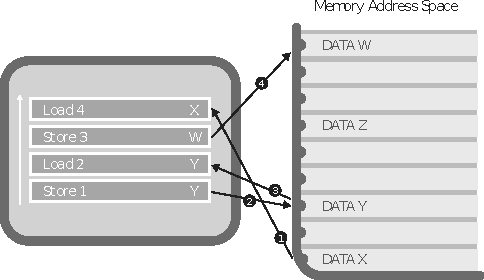
\includegraphics[width=0.6\textwidth]{methods/grayscale_memory_disambiguation.pdf}
\caption{Beispiel für eine Speicher-Disambiguierung. Die Nummern in den Kreisen geben die chronologische und der weiße Pfeil am linken Rand die logische Ausführungsreihenfolge an. Load 2 kann nicht früher ausgeführt werden, da er von Store 1 abhängig ist. Load 4 hingegen ist von den anderen Operationen unabhängig und kann daher vor Store 1 und Store 3 ausgeführt werden. Durch diese vorgezogene Ausführung können Instruktionen, die den Wert von X benötigen, im Folgenden von einer geringen Zugriffslatenz profitieren. \cite{CacheAssoWiki}.}
\end{figure}

Um diese Techniken umzusetzen, werden Store-Instruktionen bei der Ausführung nicht direkt an das Speichersystem, in diesem Fall den CPU-Cache, übermittelt.
Stattdessen werden die Store-Instrukionen inklusive der Speicheradressen und Daten in einer Store-Queue gepuffert.
Die Werte werden erst an das Speichersystem übergeben, wenn alle vorherigen Befehle im Code komplett abgeschlossen wurden.
Dies vermeidet Write-after-Read(WAR)-Konflikte, bei denen ansonsten ein früheres LOAD einen inkorrekten Wert vom Speichersystem lesen würde, weil die Ausführung eines späteren STORES vorgezogen wurde.
Auch Write-after-Write(WAW)-Konflikte werden dadurch gelöst, da keine früheren STORES ihre Werte nach späteren STORES in das Speichersystem übermitteln, wie es ohne STORE-Queue bei der Out-Of-Order-Ausführung der Fall wäre. 

Des Weiteren ermöglicht die Store-Queue die spekulative Ausführung von bedingten Verzweigungen, deren Richtung zum Ausführungszeitpunkt noch nicht bekannt ist.
Wenn ein Pfad falsch geraten wurde, muss der berechnete Pfad verworfen und alle STORES rückabgewickelt werden.
Ohne die Store-Queue wäre dies nicht möglich, da in der Zwischenzeit die geschriebenen Werte von anderen Cores gelesen sein könnten und somit der Systemzustand korrumpiert wäre.

Jedoch schafft die Store-Queue auch ein neues Problem.
Angenommen ein STORE wird ausgeführt und seine Adresse und seine Daten werden in der Store-Queue gepuffert. Kurz danach liest ein LOAD von derselben Adresse, auf die der STORE geschrieben hat.
Würde der LOAD den Wert vom Speichersystem lesen, wäre der Wert veraltet, da der im Code vorher stehende STORE noch nicht übermittelt wurde.

Um diesem Problem zu begegnen, nutzen Prozessoren in der Store-Queue die store-to-load-forwarding-Technik.
Diese veranlasst die Store-Queue, abgeschlossene STORES, die noch nicht an den Speicher übermittelt wurden, zu späteren LOADS weiterzuleiten.
Bei der Ausführung eines LOADS wird die als assoziativer Speicher umgesetzte Store-Queue nach STORES auf derselben Adresse durchsucht, welche in der logischen Ausführungsreihenfolge vorher auftauchen.
Sofern es einen Treffer gibt, wird der Wert des abgeschlossenen STORES aus der Store-Queue anstatt des veralteten Wertes aus dem Speichersystem verwendet.

Die verbesserte Eviction-Set-Suche in Abschnitt \ref{StoreFor} nutzt ein Verhalten der Speicher-Disambiguierung von Intel-Prozessoren aus.

\section{Angegriffene Hardware und Software}

Der Testrechner war ein Dell Precision T1700 mit einem Intel Core i7-4770, dessen 4 physischen Kerne beziehungsweise 8 virtuellen Kerne einen Grundtakt von 3,4GHz bieten.
Der geteilte L3-Cache ist 8 MiB groß, besitzt eine Assoziativität von 16, eine Cache-Line-Größe von 64 Byte und 8192 Cache-Sets, die in 4 Slices aufgeteilt sind.
Weiterhin ist ein Intel C226 Chipsatz und 8GB DDR3-1600 verbaut. 
Als Betriebssystem wird Ubuntu 16.04.5 LTS (GNU/Linux 4.4.0-131-generic x86_64) verwendet. 
Die getesteten Browser sind Chromium 68.0.3440.106, Firefox 62 sowie Firefox Developer Edition 63.


%Nuc i3-5... 2C4T, 

Mozilla Network Security Services(NSS) \cite{MozillaNSS} ist eine Menge von Bibliotheken, welche eine plattformübergreifende Entwicklung von sicheren Client- und Server-Anwendungen anstrebt. Dabei wird unter anderem TLS oder S/MIME implementiert. Mozilla NSS wird etwa im Firefox-Browser und der Mail-Anwendung Thunderbird eingesetzt.
Der Quellcode ist unter der Mozilla Public License verfügbar und kann online etwa im Firefox-Repository \cite{MozillaDXR} eingesehen werden.

OpenPGP ist ein Standard für das Signieren, Ver- und Entschlüsseln von Daten, welcher im RFC 4880 \cite{rfc4880} definiert wird.
OpenPGP.js \cite{OpenPGPjs} ist eine Opensource-Implementierung des OpenPGP-Protokolls in Javascript, welche sich zum Ziel gesetzt hat, OpenPGP auf einer breiten Palette von Endgeräten zu ermöglichen.
%So wird OpenPGP.js etwa vom E-Mail-Dienst Protonmail \cite{Protonmail} genutzt.

%\todo{Besser in Implementierung aufgehoben?}